%!TEX root = ../master.tex
\chapter{Background Research}\label{ch:bgresearch}



\section{Types of sources}\label{sec:typesofsources} 
The sources used in this chapter include scientific articles regarding the topic “Image to sound conversion”. The articles are published in the fields of physics, sound art and digital media. Other sources include recorded lectures of one of the articles authors.

\section{Previous work}\label{sec:previouswork}

\subsection{An experimental system for auditory image representation}\label{sec:experimentalsystem}

To interpret an image, human are naturally equipped with visual sense. However, if the visual sense is missing for an individual, the visual image is not perceivable. This allows for a technical replacement which can provide the individual with a tool to substitute the missing sense or enhance other senses which is still functional. An experimental system for vision substitution was developed by Peter B. L. Meijer. The system consists of a computer connected to a camera, which records real-time images and converts them into sound. 

The system used a method called time-multiplexed mapping, where the distribution of rows and columns in an image, the height (M) and width (N) respectively, where the pixels are stored in a matrix. The time spent scanning the image(R) is used to define when the current image ends and the next image begins. An example of this method is seen in figure \todo{Add reference}. 

\begin{figure}[!h] 
\centering
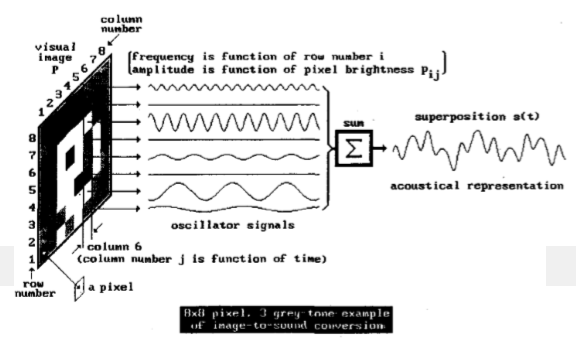
\includegraphics[width=1\textwidth]{image_to_sound}
\caption{\label{fig:image_to_sound}}
\end{figure}

\todo{add reference}
  
The images have a resolution of 64 * 64 pixels with 16 gray-tones per pixels.  

The experiment showed promising functionality to convert images to sound but lacks a field study test on people with blindness. Moreover, the advantages and disadvantages of this system is yet to be proved. This questions the reliability of the system since there is no recordings of testing data presented in the article of the experiment. However theory supports the system's functionality.  \todo{talk about the math can be used in other projects and be build upon}

\subsection{The Sound of Photographic Image}\label{sec:soundarticle}

A use of images for conversion into sound was performed and described in a paper by Atau Tanaka, who is the chair of digital media and director of culture lab at Newcastle University.

The paper describes two processing methods that both converts images into sound.

The first method utilises two image series. The method used to create the sound from the image uses a temporary mapping and additive synthesis on raw grayscale images, by scanning every pixel. A bright pixel produces high notes and a dark pixel produces a low note. \todo{Ref. paper Tanaka}

The second method was used for an interactive art installation. The interactive art consisted of a wooden structure with panels covered in rice paper to display Tanaka's pre-processed images from one of the image series. The images were processed through re-synthesis processes, where the frequency bands where quantisized to whole tones and pentatonic were mapped in which the key notes are played one at a time. The images were projected with negative pixel values creating a inverted image of the original and each row displayed different frequency ranging from low to high frequencies. An example of this result can be seen in the Figure below.  

\begin{figure}[!h]
\centering
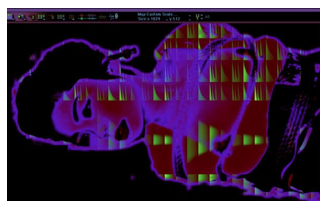
\includegraphics[width=1\textwidth]{tanakaresynthesis}
\caption{\label{fig:tanakaresynthesis}}
\end{figure}

\todo{ref to figure}

To capture human interaction, an infrared camera on top of the installation used viewers silhouettes as a layer on the negative image which was used to reveal the original black and white image for the viewer, as seen in Figure 6.

\begin{figure}[!h]
\centering
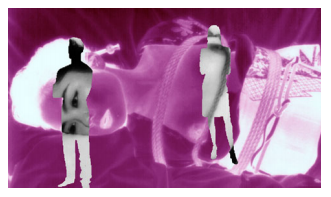
\includegraphics[width=1\textwidth]{tanakainterfacepreview}
\caption{\label{fig:tanakainterfacepreview}}
\end{figure}

\todo{ref to figure}

This interaction also affected the produced sound which were based on the brightness of the processed image and thus produced new sounds. 

This visualisation of sound through images shows dynamic functionality of a interactive system, which utilises human interaction to alter a preprossed image. However, since there was no evaluation of this exhibit, it is difficult to know of the practical application of these methods. This is due to it being used in an artistic way, instead of a practical one.   
 

\section{Methods used to evaluate}\label{sub:methodsusedtoevaluate}


\section{State of the art}\label{sec:stateart}

\subsection{Sonic Photo}\label{sub:sonic}
\todo{make into reference}
Can be found here: http://www.skytopia.com/software/sonicphoto/
!Anna rewritten!
In this project, software that allows images to be converted into sounds are to be considered as the state of the art, as they are closely related to the topic of the project. 
Sonic Photo is a free software that allows a user to input an image and converts it into a unique sounds. It !not done!




!Markus!
There are a lot of different kinds of software that allow for image to sound conversion, in this project these kind of software will be considered state of the art, as they are closely related the the topic of the project. And as it has some of the functionality that are considered to be added in the project.


Sonic photo is a free software that allows a user to input an image and convert it into sound, which can then be used for many different kind of things. It could be used by sound artists or painters to create unique sounds.

Sonic photo has many features and interface designs which are relevant to the project, which could help shape and otherwise affect the design of the project.
Sonic photo is a program that allows the user to transform an image into sound. The user can load an image into the program, and adjust various parameters to modify the resulting audio. The parameters include  frequency(Hz), brightness, tone, harmony quantization, etc.


\todo{more general information about the program. Which points to we want to make, by writing about this program?}